% Models
\chapter{Models}\label{models}
	This section defines the models we use for the different network types. We define a graph
	based representation for road and transit networks. Then both graphs are combined
	into a linked graph, making it possible to have one graph for the whole network.
	Afterwards an alternative representation for transit networks is shown.
	
% Road graph
\section{Road graph}\label{roadGraphSec}
	A road network typically is time-independent. It consists of geographical locations and roads connecting them with each other.
	We assume that a road can be taken at any time, with no time dependent constraints (see \fakesectionref{2} of \libref{networks}).
	
	Modeling the network as graph is straightforward, \defref{roadGraph} goes into detail.
	\begin{mydef}\label{roadGraph}
		A \textnormal{road graph} is a graph $G = (V, E)$ with a set of geographic coordinates
		\begin{align*}
			V = \{(\phi, \lambda) | \phi \in \left(-\frac{\pi}{2}, \frac{\pi}{2}\right), \lambda \in \left[-\pi, \pi\right)\},
		\end{align*}
		for example road junctions.
		There is an edge $(u, w, v) \in E$ iff there is a road connecting the location $u$ with the location
		$v$, which can be taken in that direction. The weight $w$ of the edge is the average time needed
		to take the road from $u$ to $v$ using a car, measured in seconds.
	\end{mydef}
	% Road graph example
	\begin{figure}[!ht]
		 \begin{center}
			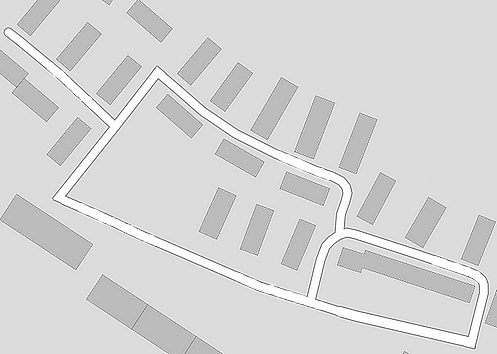
\includegraphics[scale=0.65]{res/road_network}\\
			\qquad\\
			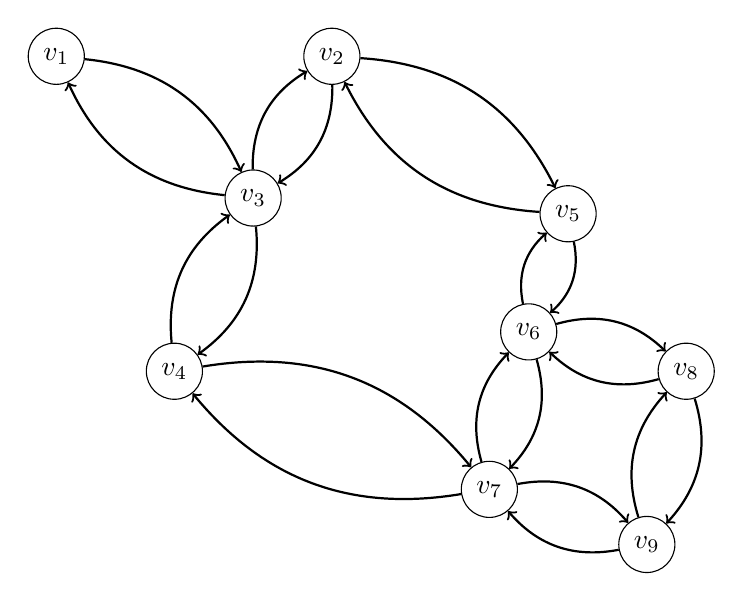
\begin{tikzpicture}[y = -1cm]
			 	% Nodes
			 	\node[circle, draw] (v1) at (0, 0) {$v_1$};
			 	\node[circle, draw] (v2) at (3.5, 0) {$v_2$};
			 	\node[circle, draw] (v3) at (2.5, 1.8) {$v_3$};
			 	\node[circle, draw] (v4) at (1.5, 4) {$v_4$};
			 	
			 	\node[circle, draw] (v5) at (6.5, 2) {$v_5$};
			 	\node[circle, draw] (v6) at (6, 3.5) {$v_6$};
			 	\node[circle, draw] (v7) at (5.5, 5.5) {$v_7$};
			 	
			 	\node[circle, draw] (v8) at (8, 4) {$v_8$};
			 	\node[circle, draw] (v9) at (7.5, 6.2) {$v_9$};
			 	
			 	% Edges
			 	\draw[thick, ->] (v1) to [bend left] (v3);
			 	\draw[thick, ->] (v3) to [bend left] (v1);
			 	
			 	\draw[thick, ->] (v3) to [bend left] (v2);
			 	\draw[thick, ->] (v2) to [bend left] (v3);
			 	\draw[thick, ->] (v3) to [bend left] (v4);
			 	\draw[thick, ->] (v4) to [bend left] (v3);
			 	
			 	\draw[thick, ->] (v2) to [bend left] (v5);
			 	\draw[thick, ->] (v5) to [bend left] (v2);
			 	\draw[thick, ->] (v4) to [bend left] (v7);
			 	\draw[thick, ->] (v7) to [bend left] (v4);
			 	
			 	\draw[thick, ->] (v5) to [bend left] (v6);
			 	\draw[thick, ->] (v6) to [bend left] (v5);
			 	\draw[thick, ->] (v6) to [bend left] (v7);
			 	\draw[thick, ->] (v7) to [bend left] (v6);
			 	
			 	\draw[thick, ->] (v6) to [bend left] (v8);
			 	\draw[thick, ->] (v8) to [bend left] (v6);
			 	\draw[thick, ->] (v7) to [bend left] (v9);
			 	\draw[thick, ->] (v9) to [bend left] (v7);
			 	
			 	\draw[thick, ->] (v8) to [bend left] (v9);
			 	\draw[thick, ->] (v9) to [bend left] (v8);
			\end{tikzpicture}
		\end{center}
		\caption{Example of a road network with its corresponding road graph. White connections indicate roads,
			dark gray rectangles represent houses or other static objects.
			Geographical coordinates for each node, as well as edge weights are omitted in the graph illustration.}
		\label{roadGraphExample}
	\end{figure}\quad\\
	\figref{roadGraphExample} shows a contrived example road network with the corresponding road graph.
	Note that two way streets result in two edges, one edge for every direction the road can be taken.\\\\
	Since edge weights are represented as average time it needs to take the road, it is possible to encode different road types.
	For example the average speed on a motorway is much higher than on a residential street. As such, the weight of an edge
	representing a motorway is much smaller than the weight of an edge representing a residential street.
	
	While the example has exactly one node per road junction this must not always be the case. Typical real world data often consists
	of multiple nodes per road segment. However, \defref{roadGraph} is still valid for such data as long as there are edges
	between the nodes if and only if there is a road connecting the locations.

% Transit graph
\section{Transit graph}\label{transitGraph}
	Transit networks can be modeled similar to road graphs. The key difference is that transit networks are time-dependent
	while road networks typically are not. For example an edge connecting \textit{Freiburg main station} with \textit{Karlsruhe main station}
	can not be taken at any time since trains and other transit vehicles only depart at certain times. The schedule might even change
	at different days.\\\\
	The difficulty lies in modeling time dependence in a static graph. There are two common approaches to that problem
	(see \libref{networks, transitModels, routePlanningOverview}).\\\\
	The first approach is called \textit{time-dependent}. There, edge weights are not static numbers but piecewise
	continuous functions that take a date with time and compute the cost it needs to take the edge when starting at the given time.
	This includes waiting time. As an example assume an edge $(u, c, v)$ with the cost function $c$. The edge represents a
	train connection and the travel time is $10$ minutes. However, the train departs at \timef{10}{15}{am}, while the starting time
	is \timef{10}{00}{am}. The cost function thus computes a waiting time of $15$ minutes plus the travel time of $10$ minutes.
	Resulting in an edge weight of $25$ minutes.
	
	The main problem with this model is that it makes pre-computations for route planning very difficult as
	the starting time is not known in advance.\\\\
	The second approach, originally from \libref{simpleTimeExpanded}, is called \textit{time-expanded}.
	There, the idea is to remove any time dependence from the graph by creating additional nodes for every
	event at a station. A node then also has a time information next to its geographic location.
	\begin{mydef}\label{simpleTransitGraph}
		A \textnormal{time expanded transit graph} is a graph $G = (V, E)$ with a set of events at geographic coordinates
		\begin{align*}
			V = \left\{\left(\phi, \lambda, t\right) \middle| \phi \in \left(-\frac{\pi}{2}, \frac{\pi}{2}\right), \lambda \in \left[-\pi, \pi\right), t \text{ time}\right\},
		\end{align*}
		for example a train arriving or departing at a train station at a certain time.
		
		For a node $v \in V$, $v_\phi$ and $v_\lambda$ denote its location and $v_t$  its time.\\\\
		There is an edge $(u, w, v) \in E$ iff
		\begin{itemize}
			\item[1.] there is a vehicle departing from $u$ at time $u_t$ which arrives at $v$ at time $v_t$ without stops in between, or
			\item[2.] $v$ is the node at the same coordinates than $u$ with the smallest time $v_t$ that is still
			greater than $u_t$. This edge represents exiting a vehicle and waiting for another connection. That is
			\begin{align*}
				\forall v' \in V \setminus \{v\}	&: v'_\phi = u_\phi \land v'_\lambda = u_\lambda \land v'_t \ge u_t\\
									&\Rightarrow v'_t - u_t > v_t - u_t.
			\end{align*}
		\end{itemize}
		The weight $w$ of an edge $(u, w, v)$ is the difference between both nodes times, that is
		\begin{align*}
			w	&= v_t - u_t.
		\end{align*}
		Note that weights are still positive since $v_t \ge u_t$ always holds due to construction.
	\end{mydef}
	% Simple transit graph example
	\begin{figure}[!ht]
		 \begin{center}
			\begin{tabular}{|c||c|cc|c|}
				\hline
				$\longrightarrow$	&\freiburg				&\multicolumn{2}{c|}{\offenburg}					&\karlsruhe\\
							&\small{\texttt{departure}}	&\small{\texttt{arrival}}		&\small{\texttt{departure}}	&\small{\texttt{arrival}}\\\hline
				\ticef			&\timef{3}{56}{pm}		&\timef{4}{28}{pm}		&\timef{4}{29}{pm}		&\timef{4}{58}{pm}\\
				\tregiof		&\timef{4}{03}{pm}		&\timef{4}{50}{pm}		&					&\\
				\tregios		&					&					&\timef{4}{35}{pm}		&\timef{5}{19}{pm}\\\hline\hline
				$\longleftarrow$	&\small{\texttt{arrival}}		&\small{\texttt{departure}}	&\small{\texttt{arrival}}		&\small{\texttt{departure}}\\\hline
				\tices			&\timef{8}{10}{pm}		&					&					&\timef{7}{10}{pm}\\\hline
			\end{tabular}\\\vphantom{a}\quad\\
			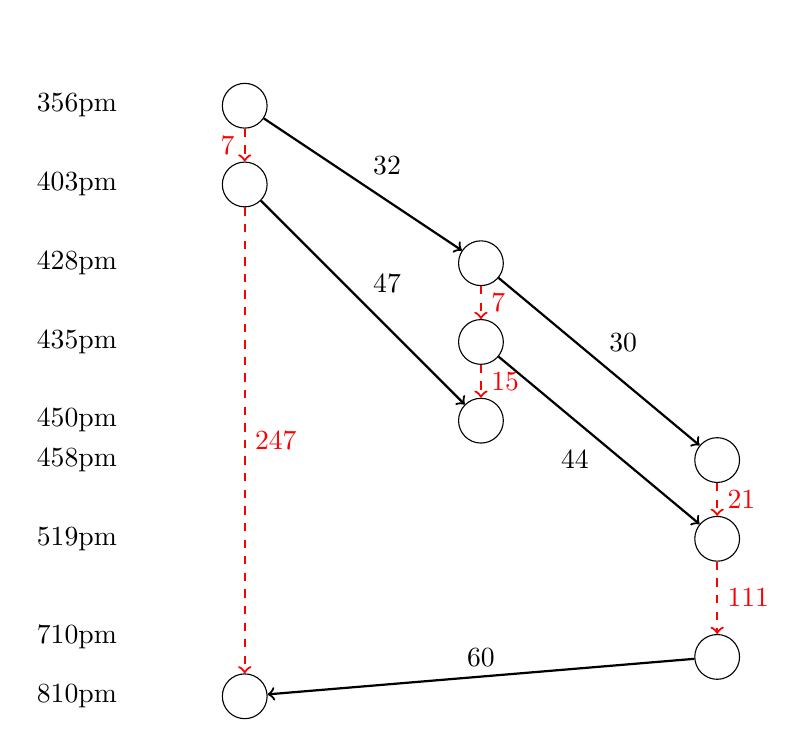
\begin{tikzpicture}[y = -1cm]
			 	% Nodes
			 	% Time line
			 	\node[left] at (-1, 0) {\timef{3}{56}{pm}};
			 	\node[left] at (-1, 1) {\timef{4}{03}{pm}};
			 	\node[left] at (-1, 2) {\timef{4}{28}{pm}};
			 	\node[left] at (-1, 3) {\timef{4}{35}{pm}};
			 	\node[left] at (-1, 4) {\timef{4}{50}{pm}};
			 	\node[left] at (-1, 4.5) {\timef{4}{58}{pm}};
			 	\node[left] at (-1, 5.5) {\timef{5}{19}{pm}};
			 	\node[left] at (-1, 6.75) {\timef{7}{10}{pm}};
			 	\node[left] at (-1, 7.5) {\timef{8}{10}{pm}};
			 	
			 	% Freiburg Hbf
			 	\node[above = 0.75cm] at (0.5, 0) {\freiburg};
			 	\node[circle, draw] (f1) at (0.5, 0) {\phantom{v}};
			 	\node[circle, draw] (f3) at (0.5, 1) {\phantom{v}};
			 	\node[circle, draw] (f4) at (0.5, 7.5) {\phantom{v}};
			 				 	
			 	% Offenburg
			 	\node[above = 0.75cm] at (3.5, 0) {\offenburg};
			 	\node[circle, draw] (o4) at (3.5, 2) {\phantom{v}};
			 	\node[circle, draw] (o2) at (3.5, 3) {\phantom{v}};
			 	\node[circle, draw] (o5) at (3.5, 4) {\phantom{v}};
			 	
			 	% Karlsruhe Hbf
			 	\node[above = 0.75cm] at (6.5, 0) {\karlsruhe};
			 	
			 	\node[circle, draw] (k3) at (6.5, 4.5) {\phantom{v}};
			 	\node[circle, draw] (k1) at (6.5, 5.5) {\phantom{v}};
			 	\node[circle, draw] (k2) at (6.5, 7) {\phantom{v}};
			 	
			 	% Edges
			 	% ICE 104
			 	\draw[thick, ->] (f1) to node[above right] {$32$} (o4);
			 	\draw[thick, ->] (o4) to node[above right] {$30$} (k3);
			 	
			 	% RE 17024
			 	\draw[thick, ->] (f3) to node[above right] {$47$} (o5);
			 	
			 	% RE 17322
			 	\draw[thick, ->] (o2) to node[below left] {$44$} (k1);
			 	
			 	% ICE 79
			 	\draw[thick, ->] (k2) to node[above] {$60$} (f4);
			 	
			 	% Waiting arcs
			 	\draw[color= red, thick, dashed, ->] (f1) to node[left] {$7$} (f3);
			 	\draw[color= red, thick, dashed, ->] (f3) to node[right] {$247$} (f4);
			 	
			 	\draw[color= red, thick, dashed, ->] (o4) to node[right] {$7$} (o2);
			 	\draw[color= red, thick, dashed, ->] (o2) to node[right] {$15$} (o5);
			 	
			 	\draw[color= red, thick, dashed, ->] (k3) to node[right] {$21$} (k1);
			 	\draw[color= red, thick, dashed, ->] (k1) to node[right] {$111$} (k2);
			\end{tikzpicture}
		\end{center}
		\caption{Example of a transit network with its corresponding time expanded transit graph.
			The table shows an excerpt of a train schedule. Regular edges indicate a train connection
			and dashed edges waiting edges. Edge weights are measured in minutes.}
		\label{simpleTransitGraphExample}
	\end{figure}\quad\\
	\defref{simpleTransitGraph} defines such a time expanded transit graph and \figref{simpleTransitGraphExample} shows an example.
	For simplicity it is assumed that the trains have no stops other than shown in the schedule. The schedule lists four trains:
	\begin{itemize}
		\item[1.] The \ticef which travels from \freiburg to \karlsruhe via \offenburg,
		\item[2.] the \tregiof connecting \freiburg with \offenburg,
		\item[3.] the \tregios driving from \offenburg to \karlsruhe and
		\item[4.] ICE \tices which travels in the opposite direction, connecting \karlsruhe with \freiburg without intermediate stops.
	\end{itemize}
	As seen in the example, the resulting graph has no time dependency anymore and is static, as well as all edge weights.
	The downside is that the graph size dramatically increases as a new node is introduced for every single event.
	In order to limit the growth, we assume that a schedule is the same every day and does not change. In fact, most schedules are
	stable and often change only slightly, for example on weekends or at holidays. In practice hybrid models can be used for
	those exceptions.\\\\
	However, the model still lacks an important feature. It does not represent \textit{transfer buffers} \libref{transitModels, routePlanningOverview} yet.
	It takes some minimal amount of time to exit a vehicle and enter a different vehicle, possibly even at a different platform.
	
	We model that by further distinguishing the nodes by arrival and departure events. In between we can then add transfer
	nodes which model the transfer duration. Therefore, the previous definition is adjusted and \defref{realisticTransitGraph} is received.
	\begin{mydef}\label{realisticTransitGraph}
		A \textnormal{realistic time expanded transit graph} is a graph $G = (V, E)$ with a set of events at geographic coordinates
		\begin{align*}
			V = \{(\phi, \lambda, t, e) | \phi \in \left(-\frac{\pi}{2}, \frac{\pi}{2}\right), \lambda \in \left[-\pi, \pi\right),
			t \text{ time}, e \in \{\arrival, \departure, \transfer\}\},
		\end{align*}
		for example a train arriving at a train station at a certain time.
		
		A node $(\phi, \lambda, t, e) \in V$ is an \textnormal{arrival node} if $e = \arrival$, analogously it is a
		\textnormal{departure node} for $e = \departure$ and a transfer node for $e = \transfer$.
		For a node $v \in V$, $v_\phi$ and $v_\lambda$ denote its location, $v_t$  its time and $v_e$ its event type.\\\\
		For every arrival node $n$ there must exist a transfer node $m$ at the same coordinates such that $m_t = n_t + d$
		with $d$ being the average transfer duration at the corresponding stop.\\\\
		There is an edge $(u, w, v) \in E$ iff
		\begin{itemize}
			\item[1.] $u_e = \departure \land v_e = \arrival$ such that there is a vehicle departing
				from $u$ at time $u_t$ which arrives at $v$ at time $v_t$ without stops in between; or
			\item[2.] $u_e = \arrival \land v_e = \departure$
				such that $u$ and $v$ belong to the same connection. For example a train arriving at a station
				and then departing again; or
			\item[3.] $u_e = \arrival \land v_e = \transfer$
				such that $v$ is the first transfer node at the same coordinates whose time $v_t$ comes after $u_t$. That is
				\begin{align*}
					\forall v' \in V \setminus \{v\}	&: v'_\phi = u_\phi \land v'_\lambda = u_\lambda \land v'_e = \transfer \land v'_t \ge u_t\\
										&\Rightarrow v'_t - u_t > v_t - u_t.
				\end{align*}
				Such an edge represents exiting the vehicle and getting ready to enter a different vehicle; or
			\item[4.] $u_e = \transfer \land v_e = \transfer$
				such that $v$ is the first transfer node at the same coordinates whose time $v_t$ comes after $u_t$,
				representing waiting at a stop; or
			\item[5.] $u_e = \transfer \land v_e = \departure$
				such that $u$ is the last transfer node at the same coordinates whose time $u_t$ comes before $v_t$, i.e.
				\begin{align*}
					\forall u' \in V \setminus \{u\}	&: u'_\phi = v_\phi \land u'_\lambda = v_\lambda \land u'_e = \transfer \land u'_t \le v_t\\
										&\Rightarrow v_t - u'_t > v_t - u_t.
				\end{align*}
				An edge like this represents entering a different vehicle from a stop after transferring or waiting at the stop.
		\end{itemize}
		The weight $w$ of an edge $(u, w, v)$ is the difference between both nodes times, that is
		\begin{align*}
			w	&= v_t - u_t.
		\end{align*}
	\end{mydef}
	% Realistic transit graph example
	\begin{figure}[!ht]
		 \begin{center}
			\begin{tikzpicture}[y = -1cm]
			 	% Nodes
			 	% Time line
			 	\node[left] at (-1, 0) {\timef{3}{56}{pm}};
			 	\node[left] at (-1, 0.75) {\timef{4}{03}{pm}};
			 	
			 	\node[left] at (-1, 1.5) {\timef{4}{28}{pm}};
			 	\node[left] at (-1, 2) {\timef{4}{29}{pm}};
			 	\node[left] at (-1, 2.75) {\timef{4}{33}{pm}};
			 	\node[left] at (-1, 3.5) {\timef{4}{35}{pm}};
			 	\node[left] at (-1, 4.25) {\timef{4}{50}{pm}};
			 	\node[left] at (-1, 5) {\timef{4}{55}{pm}};
			 	
			 	\node[left] at (-1, 5.75) {\timef{4}{58}{pm}};
			 	\node[left] at (-1, 6.5) {\timef{5}{03}{pm}};
			 	\node[left] at (-1, 7.25) {\timef{5}{19}{pm}};
			 	\node[left] at (-1, 8) {\timef{5}{24}{pm}};
			 	\node[left] at (-1, 8.75) {\timef{7}{10}{pm}};
			 	
			 	\node[left] at (-1, 9.5) {\timef{8}{10}{pm}};
			 	\node[left] at (-1, 10.25) {\timef{8}{15}{pm}};
			 	
			 	% Freiburg Hbf
			 	\node[above = 0.75cm] at (1, 0) {\freiburg};
			 	
			 	\node[minimum size=6mm, circle, draw, fill=blue!20] (f1) at (2, 0) {};
			 	
			 	\node[minimum size=6mm, circle, draw, fill=blue!20] (f3) at (2, 0.75) {};
			 	
			 	\node[minimum size=5.5mm, rectangle, draw, fill=red!20] (f4) at (0, 9.5) {};
			 	\node[minimum size=7.5mm, diamond, draw, fill=darkgreen!20] (f8) at (1, 10.25) {};
			 				 	
			 	% Offenburg
			 	\node[above = 0.75cm] at (5, 0) {\offenburg};
			 	
			 	\node[minimum size=5.5mm, rectangle, draw, fill=red!20] (o3) at (4, 1.5) {};
			 	\node[minimum size=6mm, circle, draw, fill=blue!20] (o4) at (6, 2) {};
			 	\node[minimum size=7.5mm, diamond, draw, fill=darkgreen!20] (o6) at (5, 2.75) {};
			 	
			 	\node[minimum size=6mm, circle, draw, fill=blue!20] (o2) at (6, 3.5) {};
			 	
			 	\node[minimum size=5.5mm, rectangle, draw, fill=red!20] (o5) at (4, 4.25) {};
			 	\node[minimum size=7.5mm, diamond, draw, fill=darkgreen!20] (o8) at (5, 5) {};
			 	
			 	% Karlsruhe Hbf
			 	\node[above = 0.75cm] at (9, 0) {\karlsruhe};
			 	
			 	\node[minimum size=5.5mm, rectangle, draw, fill=red!20] (k3) at (8, 5.75) {};
			 	\node[minimum size=7.5mm, diamond, draw, fill=darkgreen!20] (k5) at (9, 6.5) {};
			 	
			 	\node[minimum size=5.5mm, rectangle, draw, fill=red!20] (k1) at (8, 7.25) {};
			 	\node[minimum size=7.5mm, diamond, draw, fill=darkgreen!20] (k6) at (9, 8) {};
			 	
			 	\node[minimum size=6mm, circle, draw, fill=blue!20] (k2) at (10, 8.75) {};
			 	
			 	% Edges
			 	% ICE 104
			 	\draw[thick, ->] (f1) to node[above right] {$32$} (o3);
			 	\draw[thick, ->] (o3) to node[above] {$1$} (o4);
			 	\draw[thick, ->] (o4) to node[above right] {$29$} (k3);
			 	
			 	% RE 17024
			 	\draw[thick, ->] (f3) to node[below left] {$47$} (o5);
			 	
			 	% RE 17322
			 	\draw[thick, ->] (o2) to node[below left] {$44$} (k1);
			 	
			 	% ICE 79
			 	\draw[thick, ->] (k2) to node[above] {$60$} (f4);
			 	
			 	% Arrival to transfer
			 	\draw[color= red, thick, dashed, ->] (f4) to node[below left] {$5$} (f8);
			 	
			 	\draw[color= red, thick, dashed, ->] (o3) to node[below left] {$5$} (o6);
			 	\draw[color= red, thick, dashed, ->] (o5) to node[below left] {$5$} (o8);
			 	
			 	\draw[color= red, thick, dashed, ->] (k3) to node[above right] {$5$} (k5);
			 	\draw[color= red, thick, dashed, ->] (k1) to node[below left] {$5$} (k6);
			 	
			 	% Transfer to departure
			 	\draw[color= red, thick, dashed, ->] (o6) to node[above right] {$2$} (o2);
			 	\draw[color= red, thick, dashed, ->] (k6) to node[above right] {$106$} (k2);
			 	
			 	% Transfer to transfer
			 	\draw[color= red, thick, dashed, ->] (o6) to node[left] {$22$} (o8);
			 	
			 	\draw[color= red, thick, dashed, ->] (k5) to node[right] {$21$} (k6);
			\end{tikzpicture}
		\end{center}
		\caption{Illustration of a realistic time expanded transit graph representing the schedule from \figref{simpleTransitGraphExample}.
			A transfer duration of $5$ minutes is assumed at every stop. Rectangular nodes are arrival nodes, circular nodes
			represent departure nodes and diamond shaped nodes are transfer nodes. Regular edges indicate a train
			connection and dashed edges involve transfer nodes. Edge weights are measured in minutes.}
		\label{realisticTransitGraphExample}
	\end{figure}\quad\\
	\figref{realisticTransitGraphExample} shows how the transit graph from \figref{simpleTransitGraphExample} changes with transfer buffers.

	The weight of edges connecting arrival nodes with transfer nodes is equal to the transfer duration, $5$ minutes in the example.
	The transfer duration can be different for each edge. A transfer is now possible if the departure of the desired vehicle is after
	the arrival of the current vehicle plus the duration time. As seen in the example, edges connecting transfer nodes with departure
	nodes are present exactly in this case. A transfer from \ticef to \tregios in \offenburg is indicated by taking the edge to the
	first transfer node in \offenburg and then following the edge with cost $2$ to the departure node of the train.
% Link graph
\section{Link graph}\label{linkGraph_sec}
	In this section we examine how a road and a transit graph can be combined into a single graph such that all
	connections of the real network are preserved.\\\\
	The approach is simple, selected nodes in the road network are connected to nodes of a certain stop in
	the transit network and vice versa. Since starting time is not known in advance, the graph must connect a
	road node to all arrival nodes of a stop (compare to \libref{accessNodeRouting}).
	
	In order to not miss a connection, the transit graph must ensure that every connection starts with an arrival node.
	In \figref{realisticTransitGraphExample} this is not the case and all four trains start at a departure node. However,
	this is easily fixed by adding an additional arrival node to the beginning of every connection not starting with an arrival node already.
	The arrival nodes time is the same as the time of the departure node and both are connected by an edge with a weight of $0$.
	\defref{linkGraph} formalized the model.
	\begin{mydef}\label{linkGraph}
		Assume a road graph $R = (V_R, E_R)$, a realistic time expanded transit graph $T = (V_T, E_T)$ where
		every connection in $T$ starts by an arrival node and a partial function $\link: V_R \pto M$ where $M$
		contains subsets $S \subseteq V_T$. For every element $S \in M$ with an arbitrary element $s \in S$ the following
		properties must hold:
		\begin{itemize}
			\item[1.]
				All contained elements must be arrival nodes and have the same location than $s$, i.e.
				\begin{align*}
					\forall s' \in S: s'_e = \arrival \land s'_\phi = s_\phi \land s'_\lambda = s_\lambda.
				\end{align*}
			\item[2.]
				The set must contain all arrival nodes at the location of $s$, i.e.
				\begin{align*}
					\nexists v \in V_T \setminus S: v_e = \arrival \land v_\phi = s_\phi \land v_\lambda = s_\lambda.
				\end{align*}
		\end{itemize}
		Then, a \textnormal{link graph} is a graph $L = (V_R \cupdot V_T, E_R \cupdot E_T \cupdot E_L)$ with
		an additional set of link edges $E_L = V_R \times \mathbb{R}_{\ge 0} \times V_T$.\\\\
		There is an edge $(u, 0, v) \in E_L$ iff $\link(u)$ is defined and $v \in \link(u)$.
	\end{mydef}\quad\\
	The function $\link$ can be obtained in different ways. For example by creating a mapping from a road node $u$ to
	a stop $S$ if $u$ is in the vicinity of $S$ according to the $\asTheCrowFlies$ metric.
	
	Another straightforward possibility is to always connect a stop with the road node nearest to it. We will explore
	this problem in \sectionref{nearestNeighborProblem}. An obvious downside of this approach is that the nearest road node
	might not always have a good connectivity to the road network. A solution consists in creating a road node at the coordinates
	of the stop as representative. The node can then be connected with all road nodes in the vicinity.

% Timetable
\section{Timetable}\label{timetable_sec}
	Timetables \libref{routePlanningOverview} are non-graph based representations for transit networks.
	They consists of stops, trips, connections and footpaths.
	\begin{mydef}\label{timetable}
		A \textnormal{timetable} is a tuple $(S, T, C, F)$ with stops $S$, trips $T$, connections $C$ and footpaths $F$.
	\end{mydef}\quad\\
	A stop is a position where passengers can enter or exit a vehicle, for example a train station or bus stop.
	It is represented as geographical coordinate $(\phi, \lambda)$ with $\phi \in \left(-\frac{\pi}{2}, \frac{\pi}{2}\right),
	\lambda \in \left[-\pi, \pi\right)$.
	
	A trip is a scheduled vehicle, like the \ticef in the example schedule of \figref{simpleTransitGraphExample} or a bus.\\\\
	In contrast to a trip, a connection is only a segment of a trip without stops in between. For example the connection
	of the \ticef from \freiburg at \timef{3}{56}{pm} to \offenburg with arrival at \timef{4}{28}{pm}.
	It is defined as tuple $c = (s_{\dep}, s_{\arr}, t_{\dep}, t_{\arr}, o)$ with $s_{\dep}, s_{\arr} \in S$ representing the
	departure and arrival stop of the connection respectively. Analogously $t_{\dep}$ is the time the vehicle departs
	at $s_{\dep}$ and $t_{\arr}$ when it arrives at $s_{\arr}$. And $o \in T$ is the trip the connection belongs to.\\\\
	Footpaths represent transfer possibilities between stops and are formalized as ordered tuple $(s_{\dep}, d, s_{\arr})$ with
	$s_{\dep}, s_{\arr} \in S$ being the stops the footpath connects. The duration it needs to take the path by foot is
	represented by $d$, measured in seconds. Together with the set of stops $S$ the footpaths build a graph $G = (S, F)$,
	representing directed edges between stops.
	
	We require the following for the footpaths:
	\begin{itemize}
		\item[1.] Footpaths must be transitively closed, that is
			\begin{align*}
				\exists (a, d_1, b), (b, d_2, c) \in F \Rightarrow (a, d_3, c) \in F
			\end{align*}
			for arbitrary durations $d_1, d_2, d_3$.
		\item[2.] The triangle inequality must hold for all footpaths:
			\begin{align*}
				\exists (a, d_1, b), (b, d_2, c) \in F \Rightarrow \exists (a, d_3, c) \in F: d_3 \le d_1 + d_2
			\end{align*}
		\item[3.] Every stop must have a self-loop footpath, i.e.
			\begin{align*}
				\forall s \in S \Rightarrow (s, d, s) \in F.
			\end{align*}
			The duration $d$ models the transfer time at this stop, as already
			introduced in \sectionref{transitGraph}.
	\end{itemize}
	The first property can easily make the set of footpaths huge. However, it is necessary for our algorithms that the
	amount of footpaths stays relatively small. In practice, we therefore connect each stop only to stops in its vicinity
	and then compute the transitive closure to ensure that the model is transitively closed.\\\\
	To familiarize more with the model, we take a look at the schedule from \figref{simpleTransitGraphExample} again.
	The corresponding timetable consists of:
	\begin{align*}
		S	&= \{f, o, k\},
	\end{align*}
	where $f, o, k$ represent \freiburg, \offenburg and \karlsruhe respectively;
	\begin{align*}
		T	&= \{t_{104}, t_{17024}, t_{17322}, t_{79}\},
	\end{align*}
	representing the four trains \ticef, \tregiof, \tregios and \tices; the connections
	\begin{align*}
		&(f, o, \timef{3}{56}{pm}, \timef{4}{28}{pm}, t_{104}),\\
		&(o, k, \timef{4}{29}{pm}, \timef{4}{58}{pm}, t_{104}),\\
		&(f, o, \timef{4}{03}{pm}, \timef{4}{50}{pm}, t_{17024}),\\
		&(o, k, \timef{4}{35}{pm}, \timef{5}{19}{pm}, t_{17322}),\\
		&(k, f, \timef{7}{10}{pm}, \timef{8}{10}{pm}, t_{79})
	\end{align*}
	and at least the footpaths
	\begin{align*}
		&(f, 300, f),\\
		&(o, 300, o),\\
		&(k, 300, k)
	\end{align*}
	for transferring at the same stop with a duration of $300$ seconds ($5$ minutes).
	
	If we would decide that \offenburg is reachable from \freiburg by foot, and analogously \karlsruhe from
	\offenburg, we would also need to add a footpath connecting \freiburg directly with \karlsruhe.
	Else the footpaths would not be transitively closed anymore.